\part{Vermischtes}
\setcounter{section}{0}

\section{Trigonometrie}
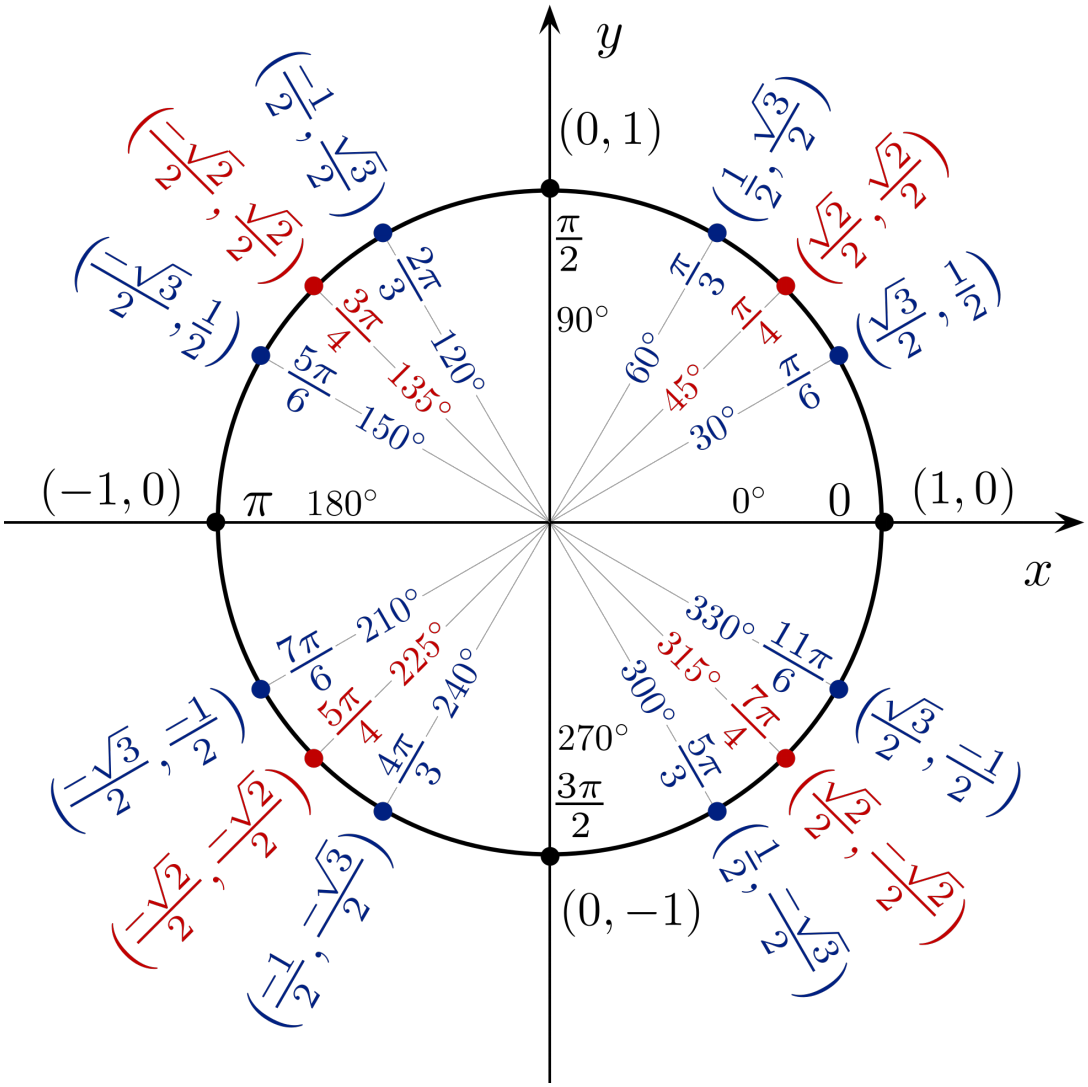
\includegraphics[scale=0.225]{sinus_cosinus}

\section{Quadratic Formula}
\[ x = \frac{-b + \pm \sqrt{b^2 - 4 a c} }{2 a} \]

\section{Proofs}
\Beweis[$\sin(x) < x$] Case distinction $\rightarrow$ Mean-Value-Theorem \\
$\forall x \in (0,1) \exists \xi \in (0,1)$ with
\begin{align*}
\sin^{\prime}(\xi) &= \frac{\sin(x)-\sin(0)}{x-0} \\
\cos(\xi)		&= \frac{\sin(x)}{x}
\end{align*}
Note that $\cos$ is bounded. \\

\Beweis[Fixpunkt 6.4a] Define $g(x):=f(x)-x \rightarrow$ Zwischenwertsatz \\

\Beweis[$1+x \leq e^x$] Bernouilli \\

\Beweis[Sandwich]
\begin{enumerate}
\item $\lim\limits_{n \rightarrow \infty} a_{n} = \lim\limits_{n \rightarrow \infty} b_{n} = \alpha$ 
\item $a_{n} \leq c_{n} \leq b_{n} \ \forall n \geq K$
\end{enumerate}

\(
\text{Es gilt } \abs{a_n - \alpha} < \epsilon \implies - \epsilon < a_n - \alpha \\
\text{Es gilt } \abs{b_n - \alpha} < \epsilon \implies + \epsilon > b_n - \alpha \\
\implies - \epsilon < a_n - \alpha \leq c_n - \alpha \leq b_n - \alpha < \epsilon \\
\implies \abs{c_n - \alpha} < \epsilon \implies \lim\limits_{n \rightarrow \infty} c_{n} = \alpha
\)

\Beweis[Hôpital]
\begin{align*}
\lim _{x \rightarrow a} \frac{f(x)}{g(x)} &=\lim _{x \rightarrow a} \frac{f(x)-f(a)}{g(x)-g(a)} \\
&=\lim _{x \rightarrow a} \frac{[f(x)-f(a)] /(x-a)}{[g(x)-g(a)] /(x-a)} \\
&=\frac{\lim _{x \rightarrow a}([f(x)-f(a)] /(x-a))}{\lim _{x \rightarrow a}([g(x)-g(a)] /(x-a))} \\
&=\frac{f^{\prime}(a)}{g^{\prime}(a)}
\end{align*}

\section{Tricks}
\Trick
\begin{align*}
a^n-b^n =& (a-b)(a^{n-1} + a^{n-2} b +\dots+b^{n-1}) \\
		=& (a-b)\sum_{i=0}^{n-1} b^{i}a^{n-1-i} 
\end{align*}

\section{Am Schluss}
\begin{itemize}
	\item 'c' nirgends vergessen?
\end{itemize}